\apendice{Especificación de diseño}

\section{Introducción}

En este apéndice se describe el diseño técnico del sistema, estructurado en tres apartados: diseño de datos, diseño arquitectónico y diseño procedimental.

El objetivo de este anexo es justificar las decisiones adoptadas durante el diseño de la solución. En particular, en el diseño de datos no solo se presenta la estructura final de la base de datos, sino también el motivo por el que se han definido determinados atributos, restricciones y relaciones. De este modo, el modelo no se plantea como una simple colección de tablas, sino como una propuesta coherente con los requisitos del sistema, la trazabilidad de la información y la posibilidad de ampliación futura.

\section{Diseño de datos}

El modelo de datos se ha diseñado para su implantación en MariaDB utilizando el motor \texttt{InnoDB}, lo que permite trabajar con claves foráneas, integridad referencial y soporte transaccional. Además, se utiliza \texttt{utf8mb4} con colación \texttt{utf8mb4\_unicode\_ci} para permitir el almacenamiento correcto de caracteres Unicode.

De manera general, el diseño se ha construido siguiendo varios criterios:

\begin{itemize}
	\item \textbf{Separación de responsabilidades}: cada tabla representa una entidad o una asociación con significado propio.
	\item \textbf{Evitar redundancia innecesaria}: se distinguen claramente conceptos como usuarios, roles, planes, suscripciones, modelos IA, modos, pipelines y ejecuciones.
	\item \textbf{Preservar la integridad}: se emplean claves primarias, claves foráneas, restricciones \texttt{UNIQUE} y restricciones \texttt{CHECK}.
	\item \textbf{Conservar la trazabilidad}: se evita el borrado automático en cascada en aquellas tablas cuyo contenido forma parte del histórico del sistema.
	\item \textbf{Facilitar la escalabilidad}: la estructura permite añadir nuevos planes, nuevos modelos IA, nuevos modos o nuevos pipelines sin modificar la base del modelo.
\end{itemize}

Antes de justificar cada una de las tablas del modelo, se incluyen dos representaciones complementarias del diseño de datos. En primer lugar, se presenta el diagrama entidad-relación, que permite comprender la estructura conceptual del sistema, sus entidades principales y las asociaciones existentes entre ellas. En segundo lugar, se muestra el diagrama del modelo relacional, donde dicha propuesta conceptual queda traducida a tablas, claves y relaciones concretas para su implantación en la base de datos.

\subsection{Diagrama entidad-relación}

La Figura~\ref{fig:diagrama_er} recoge el diagrama entidad-relación del sistema. En él se representa la visión conceptual del modelo de datos, identificando las entidades principales, sus atributos más relevantes y las relaciones que se establecen entre ellas.

\begin{figure}[H]
	\centering
	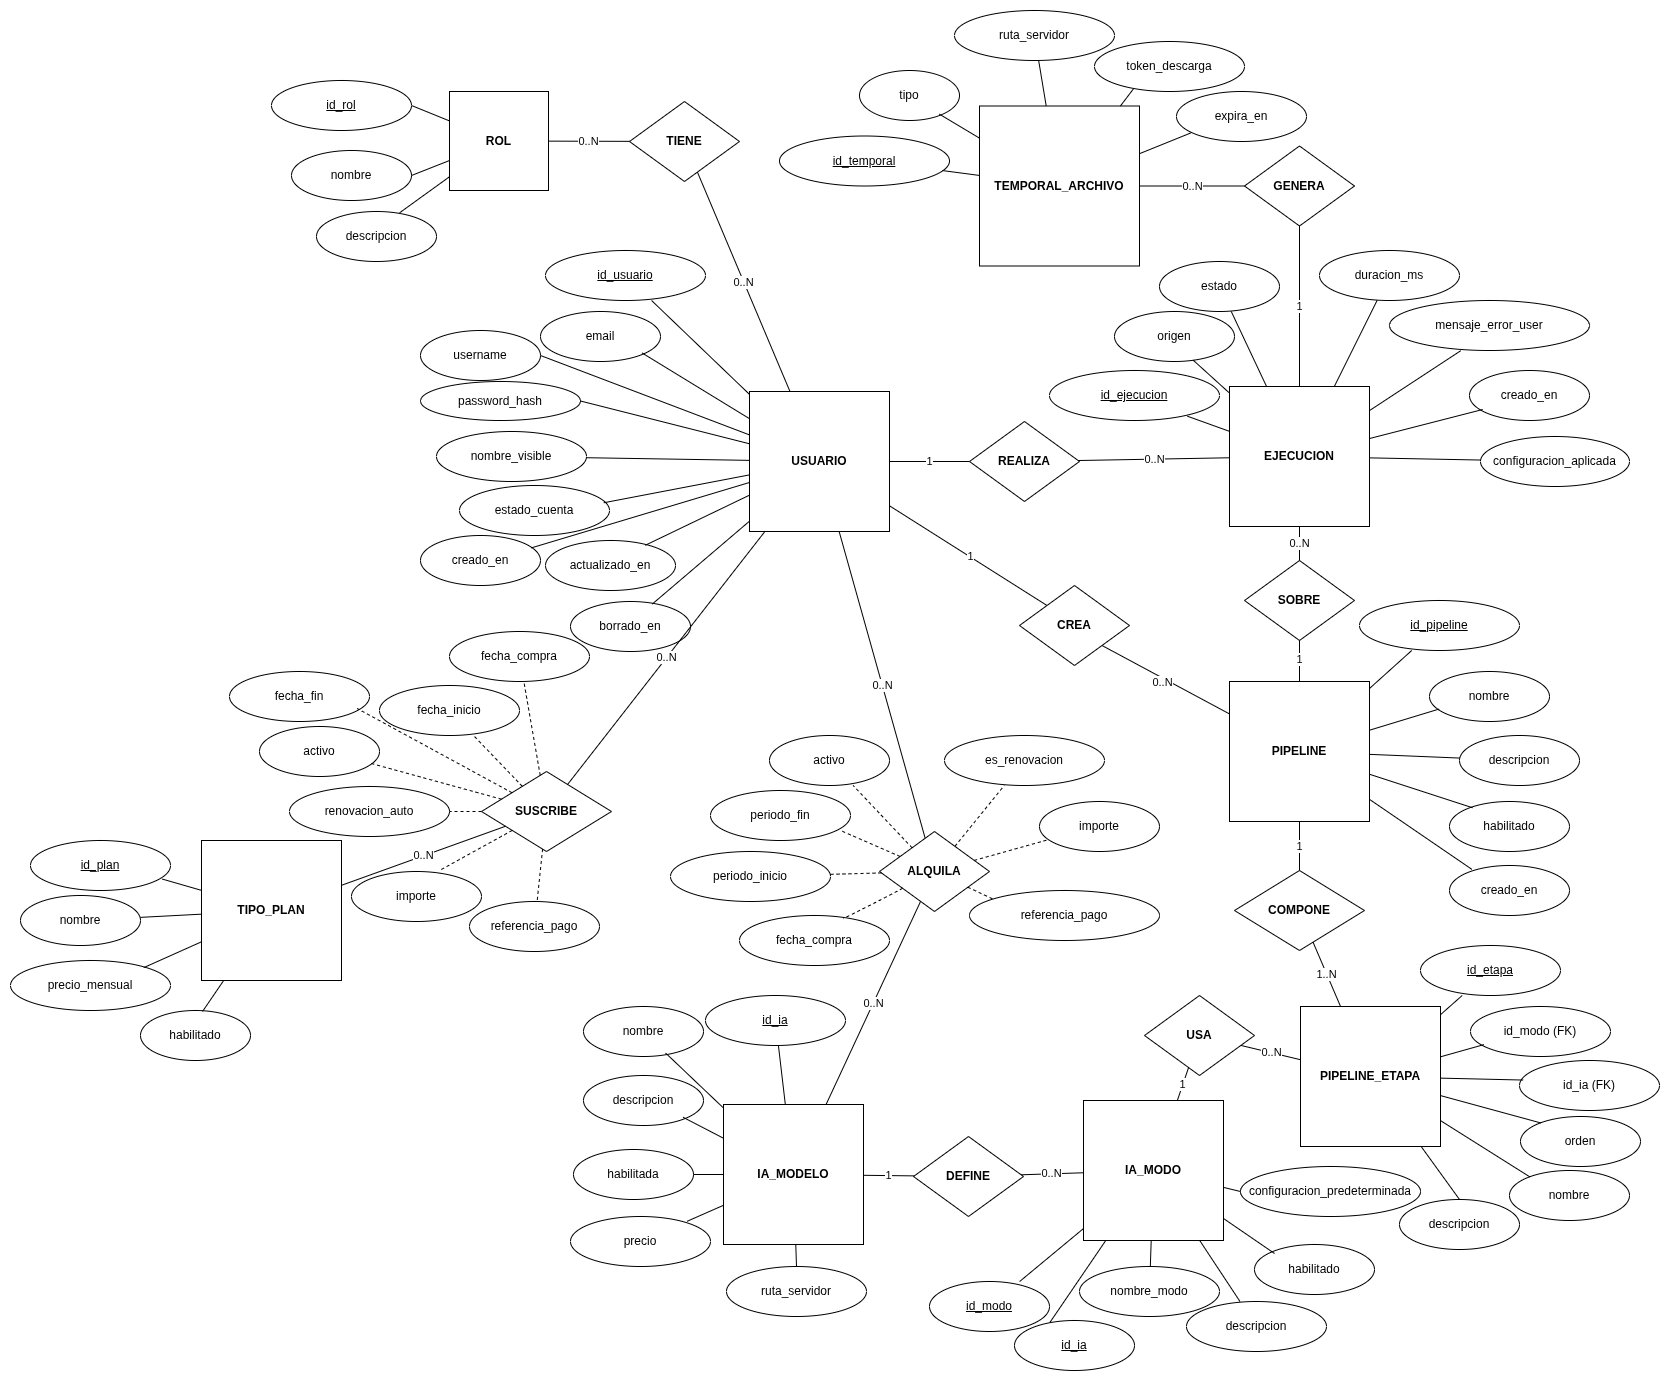
\includegraphics[width=\textwidth]{img/DiagramaModeloER.png}
	\caption{Diagrama entidad-relación del sistema}
	\label{fig:diagrama_er}
\end{figure}

Este diagrama permite observar que \texttt{USUARIO} actúa como entidad central del sistema, ya que se relaciona con la asignación de roles, la contratación de planes, el acceso individual a modelos de inteligencia artificial, la creación de pipelines y la realización de ejecuciones. Asimismo, se distingue la parte funcional asociada a los modelos IA, sus modos de uso y su composición dentro de pipelines, junto con la gestión de los archivos temporales generados durante las ejecuciones. Esta representación resulta especialmente útil para comprender el significado semántico de cada relación antes de su transformación al esquema relacional definitivo.

\subsection{Diagrama del modelo relacional}

La Figura~\ref{fig:diagrama_modelo_relacional} muestra la transformación del modelo conceptual al modelo relacional. En este nivel, las entidades y relaciones anteriores pasan a expresarse mediante tablas con sus claves primarias, claves foráneas y restricciones principales.

\begin{figure}[H]
	\centering
	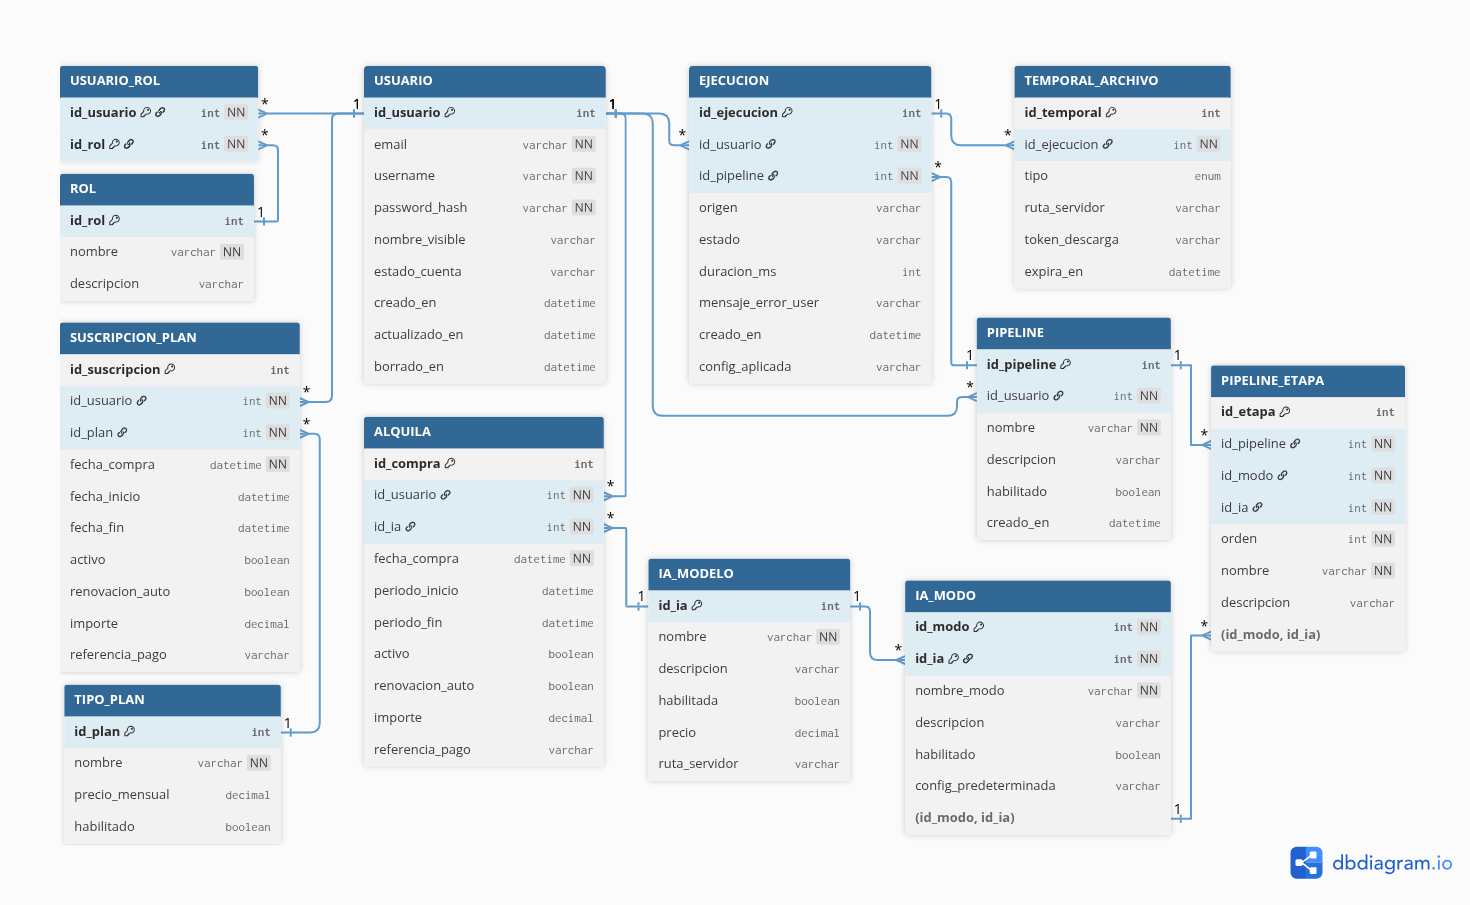
\includegraphics[width=\textwidth]{img/DiagramaModeloRelacional.png}
	\caption{Diagrama del modelo relacional del sistema}
	\label{fig:diagrama_modelo_relacional}
\end{figure}

En este diagrama puede apreciarse con mayor precisión cómo se implementan las relaciones entre las distintas tablas. Por ejemplo, las relaciones de muchos a muchos se materializan mediante tablas intermedias como \texttt{USUARIO\_ROL}, mientras que otras asociaciones se resuelven a través de claves foráneas directas, como sucede en \texttt{SUSCRIPCION\_PLAN}, \texttt{ALQUILA}, \texttt{EJECUCION} o \texttt{PIPELINE\_ETAPA}. Además, esta representación permite comprobar de forma más clara la estructura final sobre la que se aplican las restricciones de unicidad, integridad referencial y consistencia que se justifican a continuación.

A continuación se justifica cada una de las tablas del modelo..

\subsection{Tabla USUARIO}

La tabla \texttt{USUARIO} representa la cuenta de cada persona registrada en el sistema. Se trata de una tabla central, ya que gran parte del resto de entidades se relacionan directa o indirectamente con ella. Sus atributos se muestran en la Tabla~\ref{tabla:usuario_atributos}.

\tablaSmall{Atributos de la tabla USUARIO}{l p{10cm}}{usuario_atributos}
{ \multicolumn{1}{l}{Atributo} & \multicolumn{1}{l}{Descripción} \\}{
	\texttt{id\_usuario} & Identificador interno del usuario. Se define como clave primaria autoincremental para disponer de una referencia estable e independiente de los datos funcionales.\\
	\texttt{email} & Correo electrónico del usuario. Es \texttt{NOT NULL} porque constituye un dato esencial para identificar la cuenta y se declara \texttt{UNIQUE} para impedir duplicidades.\\
	\texttt{username} & Nombre de usuario del sistema. También es \texttt{NOT NULL} y \texttt{UNIQUE} porque debe existir siempre y no puede repetirse sin generar ambigüedad.\\
	\texttt{password\_hash} & Contraseña almacenada en formato hash. Es obligatoria porque forma parte de la autenticación y no se guarda en texto plano por seguridad.\\
	\texttt{nombre\_visible} & Nombre mostrado en la interfaz. Se permite \texttt{NULL} porque no es imprescindible para el funcionamiento interno del sistema.\\
	\texttt{estado\_cuenta} & Estado lógico de la cuenta. Es obligatorio y tiene el valor por defecto \texttt{activa} para evitar insertar usuarios sin estado definido.\\
	\texttt{creado\_en} & Fecha de creación del registro. Se marca como obligatoria y con valor por defecto para asegurar trazabilidad desde el alta.\\
	\texttt{actualizado\_en} & Fecha de última modificación. Se actualiza automáticamente para facilitar auditoría y seguimiento de cambios.\\
	\texttt{borrado\_en} & Fecha de borrado lógico. Se permite \texttt{NULL} porque solo debe informarse cuando el usuario deja de estar operativo sin eliminarse físicamente.\\
}

La clave primaria sobre \texttt{id\_usuario} garantiza una identificación interna única y estable. Las restricciones \texttt{UNIQUE} sobre \texttt{email} y \texttt{username} se introducen porque ambos campos tienen significado funcional dentro del sistema: el primero evita que dos cuentas compartan el mismo correo electrónico y el segundo impide colisiones en el identificador visible del usuario. Por su parte, los campos obligatorios se han limitado a los estrictamente necesarios para operar, mientras que otros como \texttt{nombre\_visible} o \texttt{borrado\_en} se mantienen opcionales para no forzar información que no siempre debe existir.

\subsection{Tabla ROL}

La tabla \texttt{ROL} almacena los distintos perfiles de acceso del sistema, como puede ser usuario administrador, cliente o futuros roles como soporte. Sus atributos se muestran en la Tabla~\ref{tabla:rol_atributos}.

\tablaSmall{Atributos de la tabla ROL}{l p{10cm}}{rol_atributos}
{ \multicolumn{1}{l}{Atributo} & \multicolumn{1}{l}{Descripción} \\}{
	\texttt{id\_rol} & Identificador interno del rol. Se utiliza una clave primaria autoincremental para desacoplar la identificación interna del nombre funcional.\\
	\texttt{nombre} & Nombre del rol. Es \texttt{NOT NULL} y \texttt{UNIQUE} para que cada rol quede claramente diferenciado y no existan duplicados lógicos.\\
	\texttt{descripcion} & Texto descriptivo del rol. Se permite \texttt{NULL} porque es útil para documentar, pero no imprescindible para aplicar permisos.\\
}

La separación de \texttt{ROL} respecto de \texttt{USUARIO} permite gestionar los perfiles de forma flexible y evita codificar los roles como un simple valor fijo dentro de la cuenta. La unicidad del nombre se justifica porque no tendría sentido disponer de dos roles con la misma denominación, ya que eso introduciría ambigüedad tanto en la lógica del sistema como en la administración.

\subsection{Tabla USUARIO\_ROL}

La tabla \texttt{USUARIO\_ROL} materializa la asignación de roles a usuarios. Sus atributos se resumen en la Tabla~\ref{tabla:usuario_rol_atributos}. Se trata de una tabla intermedia necesaria para representar una relación de muchos a muchos entre \texttt{USUARIO} y \texttt{ROL}.

\tablaSmall{Atributos de la tabla USUARIO\_ROL}{l p{10cm}}{usuario_rol_atributos}
{ \multicolumn{1}{l}{Atributo} & \multicolumn{1}{l}{Descripción} \\}{
	\texttt{id\_usuario} & Usuario al que se asigna el rol. Es obligatorio porque la asociación no tiene sentido sin un usuario existente.\\
	\texttt{id\_rol} & Rol asignado al usuario. También es obligatorio porque la asociación debe apuntar siempre a un rol concreto.\\
}

La clave primaria compuesta \texttt{(id\_usuario, id\_rol)} evita que el mismo rol se asigne varias veces al mismo usuario. Esta solución es preferible a crear un identificador artificial adicional, ya que la propia combinación de ambos campos ya identifica unívocamente la asociación. En cuanto a las acciones de borrado, se utiliza \texttt{ON DELETE CASCADE} hacia \texttt{USUARIO} porque, si un usuario desaparece, sus asignaciones dejan de tener sentido; en cambio, hacia \texttt{ROL} se usa \texttt{ON DELETE RESTRICT} para impedir eliminar un rol que todavía está siendo utilizado.


\subsection{Tabla TIPO\_PLAN}

La tabla \texttt{TIPO\_PLAN} recoge el catálogo de planes disponibles en el sistema los cuales actualmente son pro y normal teniendo pro acceso a todos los modelos de IA y normal acceso a los que alquile, además de futuros planes que se implementen. Sus atributos se presentan en la Tabla~\ref{tabla:tipo_plan_atributos}. Se separa de \texttt{SUSCRIPCION\_PLAN} para distinguir entre el tipo abstracto de plan y la contratación concreta realizada por un usuario en un periodo determinado.

\tablaSmall{Atributos de la tabla TIPO\_PLAN}{l p{10cm}}{tipo_plan_atributos}
{ \multicolumn{1}{l}{Atributo} & \multicolumn{1}{l}{Descripción} \\}{
	\texttt{id\_plan} & Identificador interno del plan. Se utiliza como clave primaria autoincremental.\\
	\texttt{nombre} & Nombre del plan. Es \texttt{NOT NULL} y \texttt{UNIQUE} porque cada elemento del catálogo debe quedar claramente identificado.\\
	\texttt{precio\_mensual} & Precio base mensual del plan. Se permite \texttt{NULL} para no obligar a informar un importe en planes gratuitos o todavía no definidos.\\
	\texttt{habilitado} & Indica si el plan está disponible para nuevas contrataciones. Es obligatorio y tiene valor por defecto \texttt{TRUE} para evitar estados indefinidos.\\
}

La restricción \texttt{UNIQUE} sobre \texttt{nombre} se justifica porque el catálogo no debe contener dos planes con la misma denominación. El \texttt{CHECK} sobre \texttt{precio\_mensual} impide valores negativos, protegiendo la coherencia del dato económico desde la propia base de datos. El campo \texttt{habilitado} permite desactivar planes sin necesidad de eliminarlos, lo que conserva referencias históricas y simplifica la administración.

\subsection{Tabla SUSCRIPCION\_PLAN}

La tabla \texttt{SUSCRIPCION\_PLAN} registra cada suscripción efectiva de un usuario a un plan concreto. Sus atributos se recogen en la Tabla~\ref{tabla:suscripcion_plan_atributos}. Se diferencia de \texttt{TIPO\_PLAN} porque aquí no se define el plan, sino cada contratación realizada.

\tablaSmall{Atributos de la tabla SUSCRIPCION\_PLAN}{l p{10cm}}{suscripcion_plan_atributos}
{ \multicolumn{1}{l}{Atributo} & \multicolumn{1}{l}{Descripción} \\}{
	\texttt{id\_suscripcion} & Identificador interno de la suscripción. Se define como clave primaria autoincremental.\\
	\texttt{id\_usuario} & Usuario suscrito. Es \texttt{NOT NULL} porque la suscripción siempre debe pertenecer a una cuenta concreta.\\
	\texttt{id\_plan} & Plan contratado. También es \texttt{NOT NULL} porque toda suscripción debe asociarse a un plan del catálogo.\\
	\texttt{fecha\_inicio} & Fecha de inicio de la suscripción. Se declara obligatoria con valor por defecto para registrar automáticamente el momento de alta.\\
	\texttt{fecha\_fin} & Fecha de finalización, cuando exista. Se permite \texttt{NULL} porque una suscripción puede estar activa o no tener todavía cierre registrado.\\
	\texttt{activo} & Indica si la suscripción está vigente. Es obligatorio y tiene valor por defecto \texttt{TRUE}.\\
	\texttt{renovacion\_auto} & Indica si la renovación es automática. Es obligatorio y se inicia en \texttt{FALSE} por defecto.\\
	\texttt{importe} & Importe cobrado en esa contratación concreta. Se permite \texttt{NULL} porque puede haber promociones o ajustes que no siempre se registren inicialmente.\\
	\texttt{referencia\_pago} & Referencia externa del pago asociado. Se deja opcional porque no tiene por qué existir siempre o puede no haberse informado todavía.\\
}

Las claves foráneas hacia \texttt{USUARIO} y \texttt{TIPO\_PLAN} usan \texttt{RESTRICT} porque las suscripciones forman parte del histórico del sistema. El \texttt{CHECK} sobre fechas impide incoherencias temporales básicas y el \texttt{CHECK} sobre \texttt{importe} evita valores negativos.

\subsection{Tabla IA\_MODELO}

La tabla \texttt{IA\_MODELO} representa cada modelo de inteligencia artificial disponible en la aplicación. Sus atributos se muestran en la Tabla~\ref{tabla:ia_modelo_atributos}. Esta tabla es una de las entidades principales del dominio, ya que el sistema se centra en permitir el acceso y la ejecución de distintos modelos IA.

\tablaSmall{Atributos de la tabla IA\_MODELO}{l p{10cm}}{ia_modelo_atributos}
{ \multicolumn{1}{l}{Atributo} & \multicolumn{1}{l}{Descripción} \\}{
	\texttt{id\_ia} & Identificador interno del modelo. Se define como clave primaria autoincremental.\\
	\texttt{nombre} & Nombre del modelo. Es \texttt{NOT NULL} y \texttt{UNIQUE} para evitar duplicidades semánticas.\\
	\texttt{descripcion} & Descripción funcional del modelo. Se permite \texttt{NULL} porque no siempre es necesaria para la lógica interna.\\
	\texttt{habilitada} & Indica si el modelo puede utilizarse. Es obligatorio y tiene valor por defecto \texttt{TRUE} para mantener un estado definido.\\
	\texttt{precio} & Coste individual del acceso al modelo, si procede. Se permite \texttt{NULL} porque algunos modelos pueden no tener precio independiente.\\
	\texttt{ruta\_servidor} & Ruta o referencia interna utilizada por el backend para localizar el modelo. Se deja opcional para no forzar que todos los modelos se resuelvan exactamente igual.\\
}

La unicidad del nombre se establece para que cada modelo tenga una identidad lógica inequívoca. El \texttt{CHECK} sobre \texttt{precio} evita importes negativos. Además, el campo \texttt{habilitada} permite activar y desactivar modelos sin eliminarlos físicamente, lo que es útil en mantenimiento, pruebas o retirada temporal del servicio.

\subsection{Tabla IA\_MODO}

La tabla \texttt{IA\_MODO} recoge los distintos modos de funcionamiento de cada modelo IA. Sus atributos aparecen en la Tabla~\ref{tabla:ia_modo_atributos}. Esta separación permite reutilizar un mismo modelo con varias configuraciones o finalidades sin necesidad de duplicarlo en la tabla principal.

\tablaSmall{Atributos de la tabla IA\_MODO}{l p{10cm}}{ia_modo_atributos}
{ \multicolumn{1}{l}{Atributo} & \multicolumn{1}{l}{Descripción} \\}{
	\texttt{id\_modo} & Identificador interno del modo. Se define como clave primaria autoincremental.\\
	\texttt{id\_ia} & Modelo al que pertenece el modo. Es \texttt{NOT NULL} porque todo modo debe estar asociado a un modelo existente.\\
	\texttt{nombre\_modo} & Nombre del modo dentro del modelo. Es obligatorio porque identifica funcionalmente la variante de uso.\\
	\texttt{descripcion} & Explicación opcional del modo. Se permite \texttt{NULL} porque no siempre será necesaria.\\
	\texttt{habilitado} & Indica si el modo está disponible para su uso. Es obligatorio y tiene valor por defecto \texttt{TRUE}.\\
	\texttt{config\_predeterminada} & Configuración base del modo. Se almacena como \texttt{TEXT} y se permite \texttt{NULL} para mantener flexibilidad y no imponer una estructura fija.\\
}

La restricción \texttt{UNIQUE (id\_ia, nombre\_modo)} evita que un mismo modelo tenga dos modos con el mismo nombre, lo que generaría ambigüedad. Además, se mantiene \texttt{UNIQUE (id\_modo, id\_ia)} porque esa combinación se usa posteriormente como referencia compuesta desde \texttt{PIPELINE\_ETAPA}. La clave foránea hacia \texttt{IA\_MODELO} utiliza \texttt{RESTRICT} para impedir eliminar un modelo si todavía conserva modos asociados.

\subsection{Tabla ALQUILA}

La tabla \texttt{ALQUILA} registra la adquisición individual de acceso a un modelo IA por parte de un usuario. Sus atributos se detallan en la Tabla~\ref{tabla:alquila_atributos}. Esta tabla resulta necesaria porque el sistema no solo contempla acceso por suscripción general, sino también compras o activaciones concretas de modelos.

\tablaSmall{Atributos de la tabla ALQUILA}{l p{10cm}}{alquila_atributos}
{ \multicolumn{1}{l}{Atributo} & \multicolumn{1}{l}{Descripción} \\}{
	\texttt{id\_compra} & Identificador interno de la operación. Se define como clave primaria autoincremental.\\
	\texttt{id\_usuario} & Usuario que realiza la compra. Es \texttt{NOT NULL} porque toda operación debe tener titular.\\
	\texttt{id\_ia} & Modelo IA adquirido. También es \texttt{NOT NULL} porque la compra debe referirse a un recurso concreto.\\
	\texttt{fecha\_compra} & Fecha de la operación. Se declara obligatoria con valor por defecto para registrar automáticamente el momento del alta.\\
	\texttt{periodo\_inicio} & Fecha de inicio de la vigencia del acceso. Se permite \texttt{NULL} porque no todas las operaciones tienen por qué estar acotadas temporalmente del mismo modo.\\
	\texttt{periodo\_fin} & Fecha de finalización de la vigencia. También se permite \texttt{NULL} para mantener flexibilidad.\\
	\texttt{activo} & Indica si el acceso está actualmente operativo. Es obligatorio y tiene valor por defecto \texttt{TRUE}.\\
	\texttt{renovacion\_auto} & Indica si la renovación del acceso es automática. Es obligatorio y se inicia por defecto en \texttt{FALSE} para no asumir renovaciones sin indicación expresa.\\
	\texttt{importe} & Importe cobrado en la operación concreta. Es necesario para si cambia el precio de alquiler de modelo quede registrado cuando se pagó en el momento de la compra. Se permite \texttt{NULL} porque puede haber casos gratuitos, promocionales o pendientes de registrar.\\
	\texttt{referencia\_pago} & Referencia externa del pago. Se deja opcional porque no siempre existirá una referencia única o puede no haberse informado todavía.\\
}

Las claves foráneas hacia \texttt{USUARIO} e \texttt{IA\_MODELO} emplean \texttt{RESTRICT} porque estas operaciones forman parte del histórico de negocio y no conviene perderlas automáticamente al eliminar entidades relacionadas. El \texttt{CHECK} sobre \texttt{importe} evita cantidades negativas y el \texttt{CHECK} sobre el periodo obliga a que, si ambas fechas existen, la fecha final no sea anterior a la inicial.

\subsection{Tabla PIPELINE}

La tabla \texttt{PIPELINE} representa un flujo de procesamiento configurable. Sus atributos se presentan en la Tabla~\ref{tabla:pipeline_atributos}. En el diseño final destaca especialmente que el campo \texttt{id\_usuario} puede ser nulo y que, si el usuario se elimina, su valor pasa a \texttt{NULL} en lugar de desaparecer el pipeline esto es debido a que si se crea un pipeline por un administrador y se elimina dicho usuario no tiene sentido que dejen de existir sus pipelines creados
.

\tablaSmall{Atributos de la tabla PIPELINE}{l p{10cm}}{pipeline_atributos}
{ \multicolumn{1}{l}{Atributo} & \multicolumn{1}{l}{Descripción} \\}{
	\texttt{id\_pipeline} & Identificador interno del pipeline. Se define como clave primaria autoincremental.\\
	\texttt{id\_usuario} & Usuario propietario del pipeline. Se permite \texttt{NULL} porque el diseño contempla conservar el pipeline aunque desaparezca su propietario original.\\
	\texttt{nombre} & Nombre del pipeline. Es \texttt{NOT NULL} porque resulta necesario para identificarlo funcionalmente.\\
	\texttt{descripcion} & Descripción del flujo. Se permite \texttt{NULL} porque no siempre es imprescindible documentarlo.\\
	\texttt{habilitado} & Indica si el pipeline puede utilizarse. Es obligatorio y tiene valor por defecto \texttt{TRUE}.\\
	\texttt{creado\_en} & Fecha de creación del pipeline. Se registra automáticamente para mantener trazabilidad temporal.\\
}

La restricción \texttt{UNIQUE (id\_usuario, nombre)} evita que un mismo usuario tenga dos pipelines con el mismo nombre, lo que simplifica la gestión y evita ambigüedades. El hecho de permitir \texttt{NULL} en \texttt{id\_usuario} y usar \texttt{ON DELETE SET NULL} responde a una decisión de conservación: si el usuario desaparece, el pipeline puede seguir existiendo como estructura lógica. No se utiliza \texttt{CASCADE} porque eso implicaría perder pipelines potencialmente reutilizables o relevantes para el histórico del sistema.


\subsection{Tabla EJECUCION}

La tabla \texttt{EJECUCION} registra cada ejecución concreta realizada en el sistema. Sus atributos se muestran en la Tabla~\ref{tabla:ejecucion_atributos}. Esta tabla es clave para la trazabilidad operativa, ya que permite saber quién ejecutó qué, cuándo lo hizo y con qué resultado.

\tablaSmall{Atributos de la tabla EJECUCION}{l p{10cm}}{ejecucion_atributos}
{ \multicolumn{1}{l}{Atributo} & \multicolumn{1}{l}{Descripción} \\}{
	\texttt{id\_ejecucion} & Identificador interno de la ejecución. Se define como clave primaria autoincremental.\\
	\texttt{id\_usuario} & Usuario asociado a la ejecución. Es obligatorio para mantener responsabilidad y trazabilidad.\\
	\texttt{id\_pipeline} & Pipeline ejecutado. Es \texttt{NOT NULL} porque cada ejecución debe quedar vinculada a un flujo concreto.\\
	\texttt{origen} & Punto de entrada desde el que se lanza la ejecución. Se permite \texttt{NULL} porque no siempre es necesario registrar esta información.\\
	\texttt{estado} & Estado de la ejecución. Es obligatorio y su valor por defecto es \texttt{pendiente}, que representa el estado inicial natural.\\
	\texttt{duracion\_ms} & Duración de la ejecución en milisegundos. Se permite \texttt{NULL} porque puede no conocerse todavía al inicio del proceso.\\
	\texttt{mensaje\_error\_user} & Mensaje de error orientado al usuario. Es opcional porque solo se utiliza cuando la ejecución falla.\\
	\texttt{creado\_en} & Fecha de creación de la ejecución. Se registra automáticamente para mantener trazabilidad temporal.\\
	\texttt{config\_aplicada} & Configuración real utilizada en la ejecución. Se permite \texttt{NULL} porque no siempre será necesario persistirla.\\
}

La clave foránea hacia \texttt{USUARIO} utiliza \texttt{RESTRICT} para no perder histórico operativo al eliminar usuarios. La clave foránea hacia \texttt{PIPELINE} también usa \texttt{RESTRICT}, lo que implica que no se puede eliminar un pipeline si existen ejecuciones asociadas a él. Esta decisión se justifica porque una ejecución debe seguir apuntando al pipeline concreto con el que fue lanzada y no conviene dejar esa referencia incompleta. El \texttt{CHECK} sobre \texttt{duracion\_ms} evita registrar tiempos negativos.

\subsection{Tabla TEMPORAL\_ARCHIVO}

La tabla \texttt{TEMPORAL\_ARCHIVO} gestiona los archivos temporales asociados a una ejecución. Sus atributos aparecen en la Tabla~\ref{tabla:temporal_archivo_atributos}. Estos recursos pueden representar archivos de entrada, de salida o intermedios y su naturaleza es claramente dependiente de la ejecución que los genera.

\tablaSmall{Atributos de la tabla TEMPORAL\_ARCHIVO}{l p{10cm}}{temporal_archivo_atributos}
{ \multicolumn{1}{l}{Atributo} & \multicolumn{1}{l}{Descripción} \\}{
	\texttt{id\_temporal} & Identificador interno del archivo temporal. Se define como clave primaria autoincremental.\\
	\texttt{id\_ejecucion} & Ejecución a la que pertenece el archivo. Es obligatorio porque el temporal no tiene sentido de forma independiente.\\
	\texttt{tipo} & Tipo de archivo temporal. Se permite \texttt{NULL} porque puede haber casos en los que no se clasifique expresamente.\\
	\texttt{ruta\_servidor} & Ruta interna del archivo en el servidor. Se deja opcional para no imponer una única forma de gestión.\\
	\texttt{token\_descarga} & Token utilizado para acceso o descarga controlada. Se permite \texttt{NULL} porque no todos los archivos temporales tienen por qué exponerse.\\
	\texttt{expira\_en} & Fecha de expiración del recurso temporal. Es opcional porque puede calcularse o no utilizarse en todos los casos.\\
}

La restricción \texttt{UNIQUE} sobre \texttt{token\_descarga} garantiza que, si existe, cada token identifique un único recurso. La clave foránea hacia \texttt{EJECUCION} emplea \texttt{ON DELETE CASCADE} porque aquí sí existe una dependencia total: si desaparece la ejecución, carece de sentido conservar sus archivos temporales. Es precisamente un caso claro y justificado de borrado en cascada.

\subsection{Tabla PIPELINE\_ETAPA}

La tabla \texttt{PIPELINE\_ETAPA} descompone cada pipeline en etapas ordenadas. Sus atributos se muestran en la Tabla~\ref{tabla:pipeline_etapa_atributos}. Esta estructura permite representar un procesamiento secuencial y modular, en el que cada etapa invoca un modo concreto de un modelo IA.

\tablaSmall{Atributos de la tabla PIPELINE\_ETAPA}{l p{10cm}}{pipeline_etapa_atributos}
{ \multicolumn{1}{l}{Atributo} & \multicolumn{1}{l}{Descripción} \\}{
	\texttt{id\_etapa} & Identificador interno de la etapa. Se define como clave primaria autoincremental.\\
	\texttt{id\_pipeline} & Pipeline al que pertenece la etapa. Es obligatorio porque una etapa no existe de forma autónoma.\\
	\texttt{id\_modo} & Modo IA utilizado en la etapa. Es \texttt{NOT NULL} porque la etapa debe invocar una operación concreta.\\
	\texttt{id\_ia} & Modelo IA asociado al modo referenciado. Es obligatorio para reforzar la coherencia de la referencia compuesta.\\
	\texttt{orden} & Posición de la etapa dentro del pipeline. Es obligatorio porque el flujo debe tener un orden definido.\\
	\texttt{nombre} & Nombre de la etapa. Es obligatorio para identificarla funcionalmente dentro del flujo.\\
	\texttt{descripcion} & Descripción opcional de la finalidad de la etapa. Se permite \texttt{NULL} porque no siempre será necesaria.\\
}

La clave foránea hacia \texttt{PIPELINE} utiliza \texttt{ON DELETE CASCADE} porque las etapas dependen completamente del pipeline al que pertenecen. En cambio, la clave foránea compuesta \texttt{(id\_modo, id\_ia)} hacia \texttt{IA\_MODO} usa \texttt{RESTRICT} para impedir eliminar un modo que todavía está siendo utilizado. La restricción \texttt{UNIQUE (id\_pipeline, nombre, orden)} evita duplicidades problemáticas dentro de un mismo pipeline, y el \texttt{CHECK (orden >= 1)} obliga a que el orden sea positivo y coherente con la idea de secuencia.

\subsection{Relaciones del modelo}

Una vez descritas las tablas por separado, conviene explicar de forma conjunta las relaciones del modelo para entender mejor el sentido global del diseño.

\begin{itemize}
	\item \textbf{USUARIO -- USUARIO\_ROL -- ROL}: la asignación de roles se resuelve mediante una tabla intermedia porque la relación es de muchos a muchos. Un usuario puede tener varios roles y un rol puede estar asignado a varios usuarios.
	
	\item \textbf{USUARIO -- SUSCRIPCION\_PLAN}: un usuario puede contratar varias suscripciones a lo largo del tiempo, mientras que cada suscripción pertenece a un único usuario.
	
	\item \textbf{TIPO\_PLAN -- SUSCRIPCION\_PLAN}: un tipo de plan puede estar asociado a muchas suscripciones, mientras que cada suscripción corresponde a un único plan.
	
	\item \textbf{USUARIO -- ALQUILA}: un usuario puede realizar múltiples compras individuales de modelos IA, pero cada operación pertenece a un único usuario.
	
	\item \textbf{IA\_MODELO -- ALQUILA}: un modelo IA puede aparecer en muchas compras individuales, mientras que cada compra referencia a un único modelo.
	
	\item \textbf{IA\_MODELO -- IA\_MODO}: un modelo puede disponer de varios modos, mientras que cada modo pertenece a un único modelo.
	
	\item \textbf{USUARIO -- PIPELINE}: un usuario puede crear varios pipelines. Sin embargo, se permite que el pipeline sobreviva a la eliminación de su propietario mediante \texttt{ON DELETE SET NULL}. Esta decisión favorece la conservación de la estructura del flujo sin vincular su existencia estrictamente al usuario original.
	
	\item \textbf{PIPELINE -- PIPELINE\_ETAPA}: un pipeline puede contener varias etapas y estas dependen totalmente de él, por eso se utiliza borrado en cascada.
	
	\item \textbf{IA\_MODO -- PIPELINE\_ETAPA}: cada etapa referencia un modo concreto mediante la pareja \texttt{(id\_modo, id\_ia)}. Esta referencia compuesta garantiza que el modo utilizado pertenece realmente al modelo indicado.
	
	\item \textbf{USUARIO -- EJECUCION}: un usuario puede generar muchas ejecuciones, mientras que cada ejecución pertenece a un único usuario.
	
	\item \textbf{PIPELINE -- EJECUCION}: un pipeline puede ejecutarse muchas veces. En el diseño final se utiliza \texttt{RESTRICT} porque se considera importante que cada ejecución mantenga la referencia completa al pipeline con el que fue lanzada.
	
	\item \textbf{EJECUCION -- TEMPORAL\_ARCHIVO}: una ejecución puede generar varios archivos temporales y cada archivo temporal pertenece a una única ejecución. Aquí sí se justifica claramente el borrado en cascada, ya que el temporal depende por completo de la ejecución.
\end{itemize}

\subsection{Valoración global del modelo}

En conjunto, el modelo de datos final busca equilibrio entre flexibilidad, integridad y conservación del histórico. Las restricciones \texttt{UNIQUE} evitan duplicidades funcionales, los \texttt{CHECK} impiden valores inválidos sencillos y las claves foráneas mantienen la coherencia entre entidades. Además, la elección entre \texttt{CASCADE}, \texttt{RESTRICT} y \texttt{SET NULL} no se ha hecho de manera uniforme, sino en función del significado de cada relación dentro del sistema.

De este modo, el modelo no solo representa correctamente las entidades del dominio, sino que también refleja decisiones de diseño orientadas a la robustez, la trazabilidad y la mantenibilidad de la aplicación.

\section{Diseño arquitectónico}

\section{Diseño procedimental}